\documentclass{article}
\begin{document}
\large
\section{Market analysis}
    \subsection{Target market}
       % The target market is parents of children with ADHD or young professionals in stationary office jobs diagnosed with ADHD. The target market is thus interested to alleviate their ADHD symptoms while keeping their hands free, in order to engage in school activities or to remain effective at work.

        The target market are young professionals who are diagnosed with ADHD and want to alleviate their symptoms while remaining effective in their stationary office jobs. They want to do so discretely and professionally, while keeping their hands free. They want a product that is portable and easy to set up. The market can be further narrowed by considering their socioeconomic status, age and income,

        \begin{table}[htbp]
            \centering
            \caption{Tabulation of target market}
            \begin{tabular}{c|c}
                \hline
                 Socioeconomic status   & Middle and upper class  \\
                 Income                 & upwards of R 50 000 \\
                 Age                    & 18 to 40\\
                 Profession             & Any office occupation\\
                 Personality trait      & Professionals diagnosed with ADHD\\
                 \hline
            \end{tabular}
            
            \label{tab:market}
        \end{table}

        As seen in Table \ref{tab:market}, lower income persons are not considered since they do not tend to work stationary office jobs. Older professionals are also not included, since ADHD symptoms are more prevalent in younger professionals. The product is intended to target individuals who are willing to spend more on a product with a professional aesthetic and superior portability. 
       
    \subsection{Market maps to identify market gap}
    \begin{figure}[H]
        \centering
        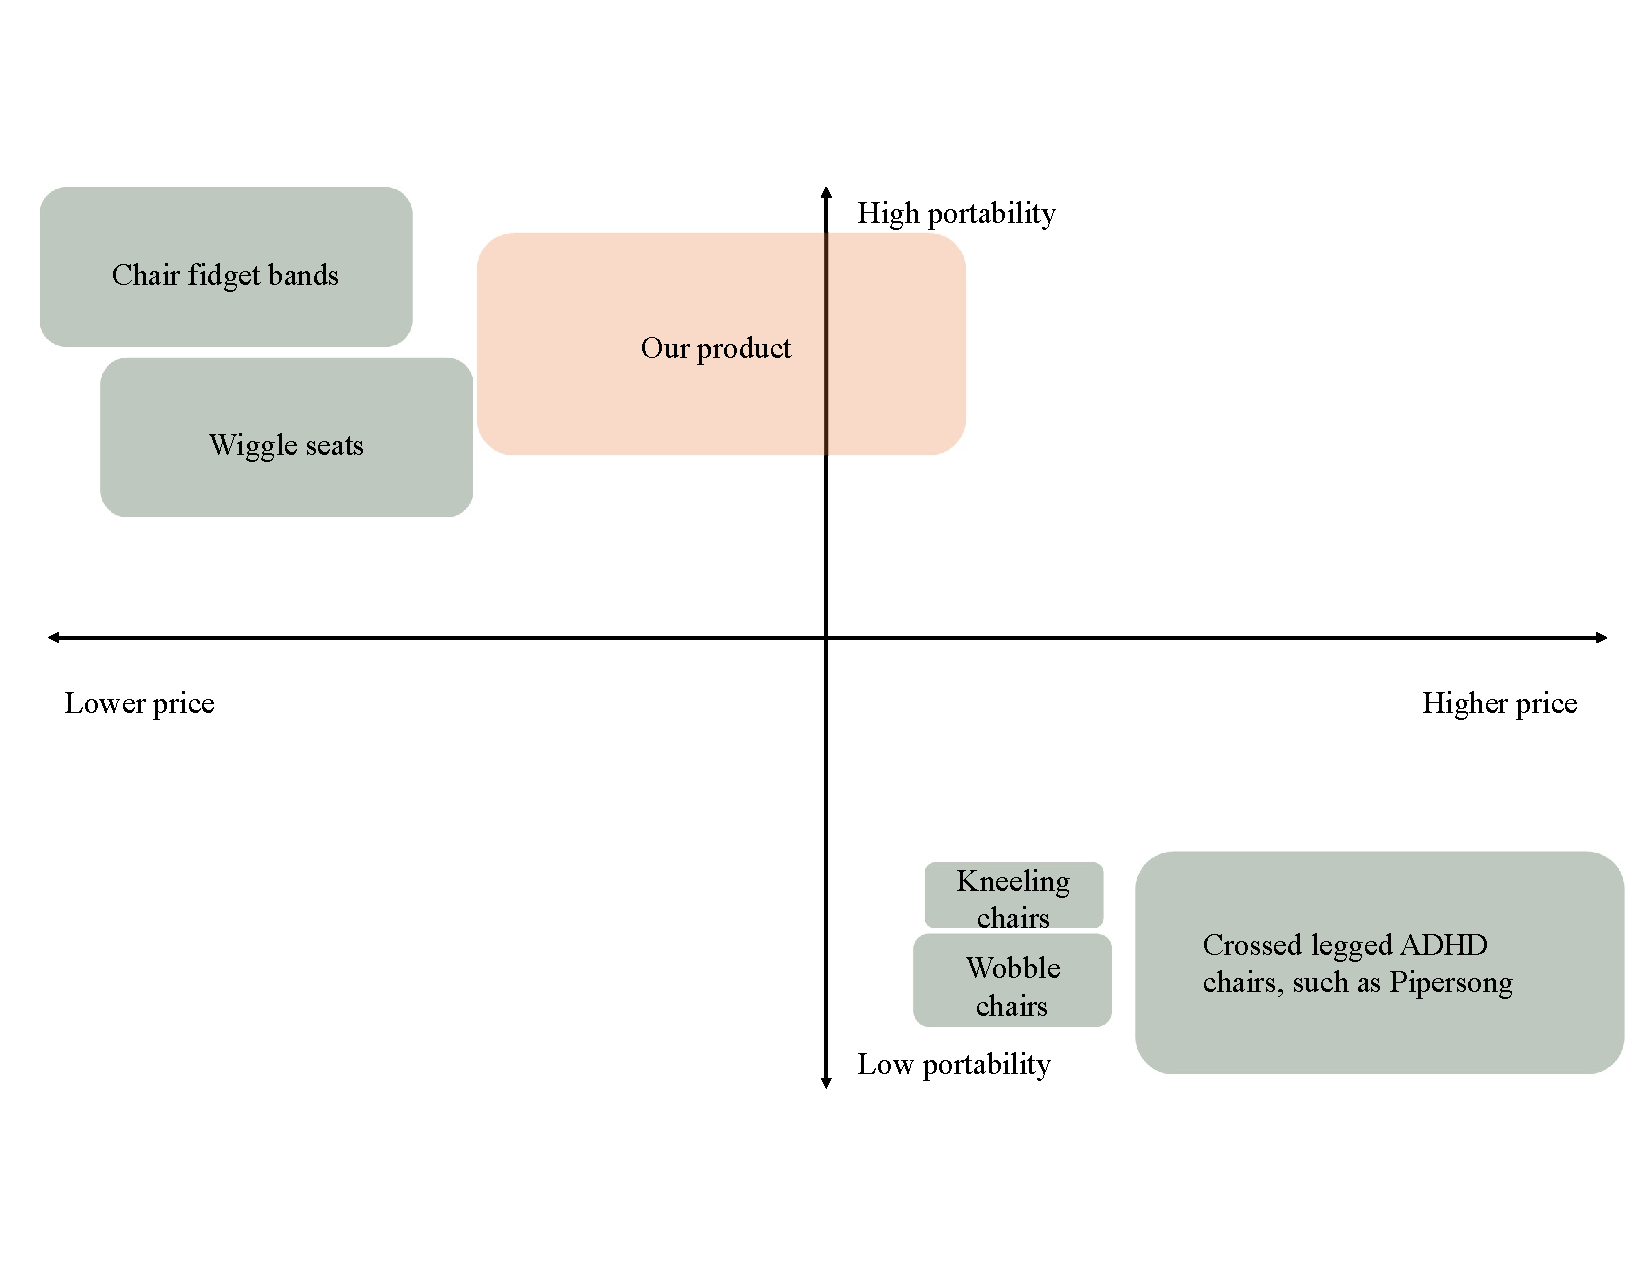
\includegraphics[width=0.75\linewidth]{figures/Map1.pdf}
        \caption{Market map of product types compared by price and portability}
        \label{fig:map1}
    \end{figure}

    Many different product types exist which allows the consumer alleviate their ADHD symptoms hands free without distracting others. The product types can be further characterized by their portability and aesthetic. Figure \ref{fig:map1}, compares the different product types by price and mobility. There is a notable gap in higher priced and portable products. However, to remain competitive the proposed product must be fairly priced in comparison to other portable products.

    Figure \ref{fig:map2} compares products to their aesthetic (how professional it appears) to its price. There is a significant gap in professional yet economic products. 

    \begin{figure}[htbp]
        \centering
        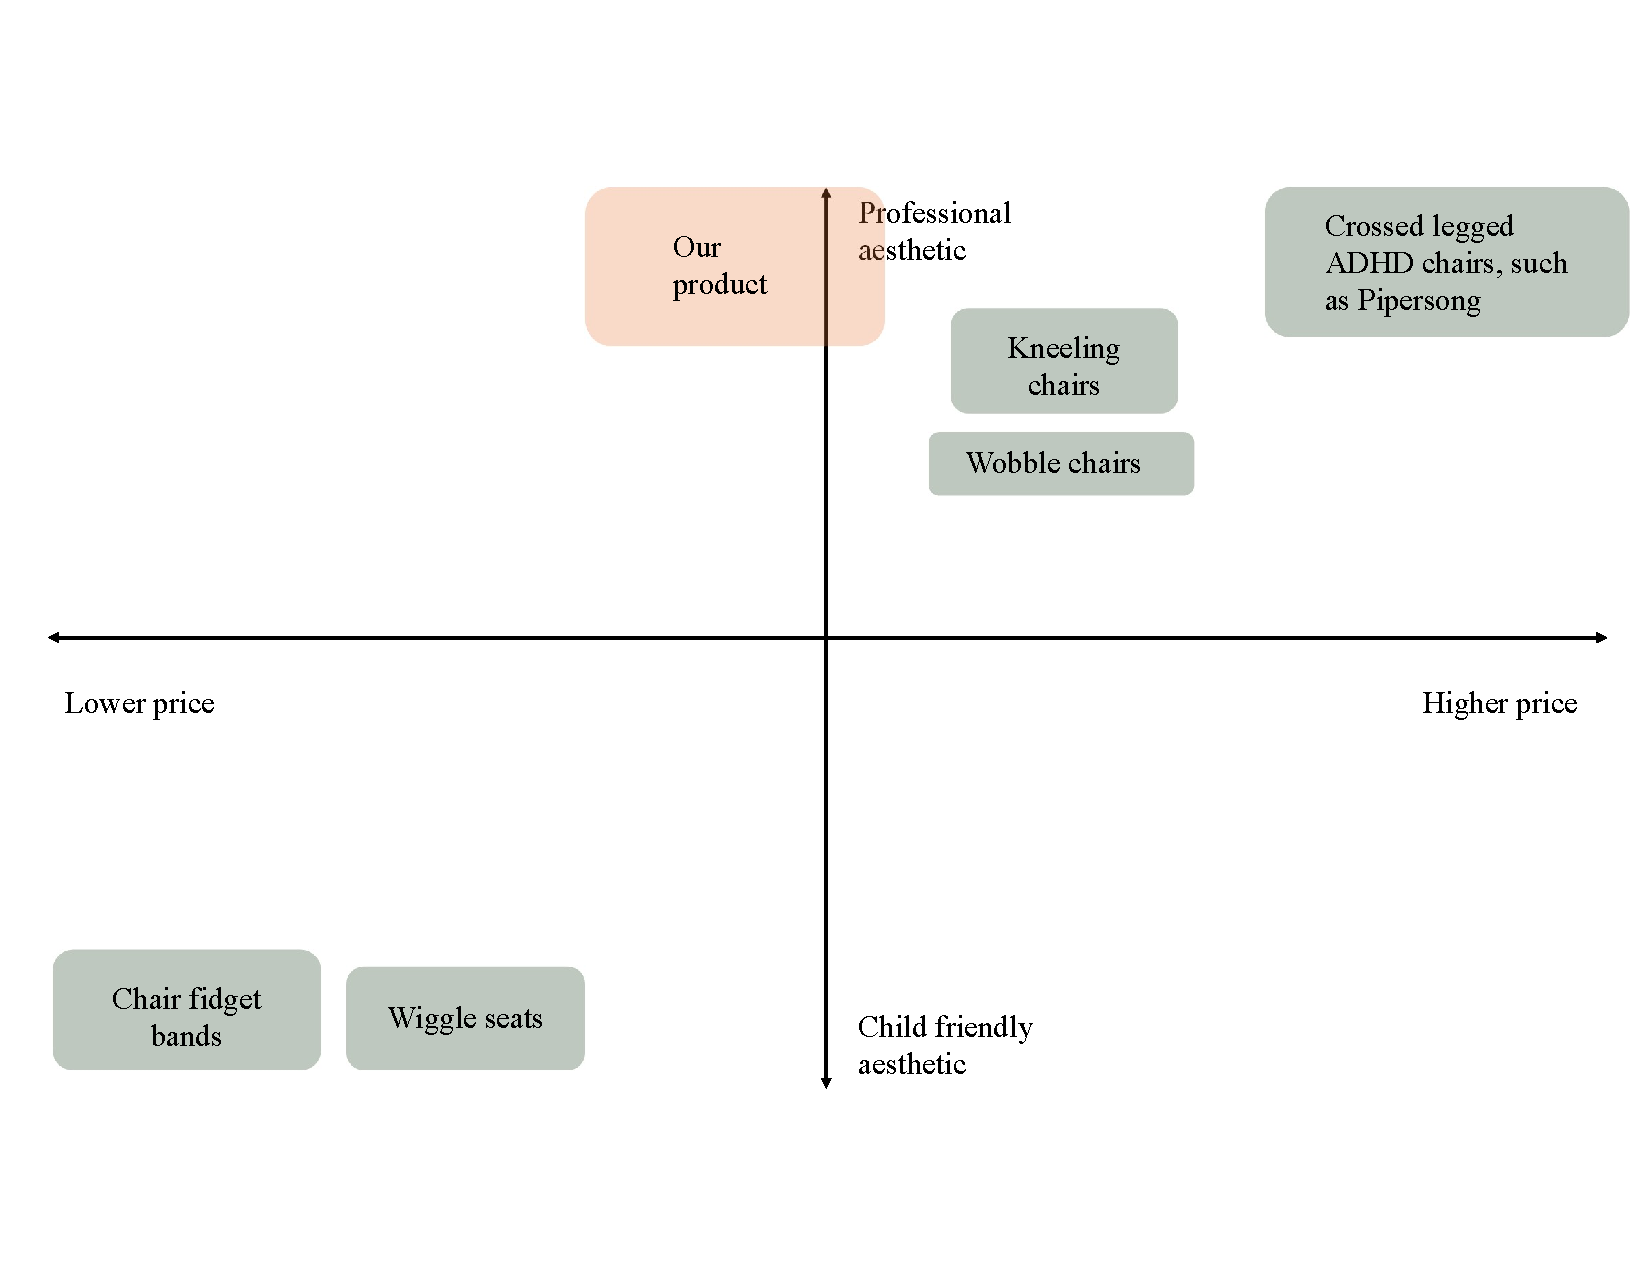
\includegraphics[width=0.75\linewidth]{figures/Map2.pdf}
        \caption{Market map of product types compared by price and aesthetic}
        \label{fig:map2}
    \end{figure}
    
    \subsection{Porter's market forces}
    In order to determine market viability and profitability of the business, all five of Porter's market forces need to be analysed, namely competitive rivalry, supplier power, buyer power, threat of substitution, and threat of new entry.
    \subsubsection{Competitive rivals}
    The main competitors to the proposed products are the producers of Wiggle Seats and chair fidget bands. This is due to similar level of portability these products offer. The competition these products bring increases if the proposed product cannot be priced relatively close to those products. Low prices will outweigh the more professional aesthetic the proposed products offers. 
    \subsubsection{Supplier power}
    Suppliers influence the decision of materials and price point of the product. If the scarcity of a certain material outweighs the value it adds to the product, it should not be used as this could negatively affect the supply chain. Similarly, if the suppliers increase the cost of the materials they supply, the profitability of our product decreases. Thus choosing readily available materials need to be taken into account when designing the product, inorder to reduce the bargaining power of the supplier.
    
    \subsubsection{Buyer power}
    The buyer has the choice of selecting a product that best suites their individual needs. The product must be positioned in a way that it ensures a unique solution to the problem, where the competitors do not overshadow the proposed product. The proposed entry point shown in Figure \ref{fig:map1} and \ref{fig:map2}, is ideal. The product will be more or equally portable than the competitors and be more professionally appropriate for white collar workers. Buyers also has the power to demand a lower price, if the perceived value of the product is lower than the selling price. 
    

   % \subsubsection{Threats}
    \subsubsection{Threat of substitution}
    There exists a threat of substitution from Wiggle seats, since if the enhanced portability and more professional aesthetic is not evident to the consumer or the price is not comparatively competitive, they might substitute the product for a wiggle seat that provides the same hands-free ADHD relief.
    \subsubsection{Threat of new entry}
    It is possible that new entrants also offers a more professional or portable product of the same category, it is then necessary to re-evaluate the product's position and improve where needed.

    \subsection{Value Proposition}
    Considering the five forces mentioned above, the proposed product above is a portable, ADHD seat attachment. The main values of the product is the focus on portability and the office appropriate aesthetic that blends in seamlessly. 

    The portability allows the consumer to relieve their ADHD symptoms in their work environment and at home with minimal effort to transport the product. The hands-free, noise free design allows the consumer to focus on tasks effectively, without causing disturbances to others. The office appropriate aesthetic allows the product to blend into the office environment.
\end{document}
